\section{EXE 1 - RA}
\begin{itemize}
	\item Pulita disposizione dei record di attivazione: disposti lateralmente, per riprendere la crescita verso il basso dello stack;
	\item Eliminata la colorazione delle variabili che rappresentavano riferimento alla stessa area di memoria (quando si ha passaggio per riferimento, come nel caso della funzione \textit{f(int x, int \&y)} in cui il parametro y viene passato per riferimento);
\end{itemize}

Nella figura ~\ref{fig:ra}, si vede una visione d'insieme (parziale) della correzione dell'esercizio 1, in cui si è seguita una linea di crescita \textit{verticale}, proprio come la memoria stack: in particolare, la \textbf{crescita laterale rappresenta lo sviluppo nel tempo della memoria}, al seguirsi delle varie istruzioni.
\begin{figure}[h]
	\centering
	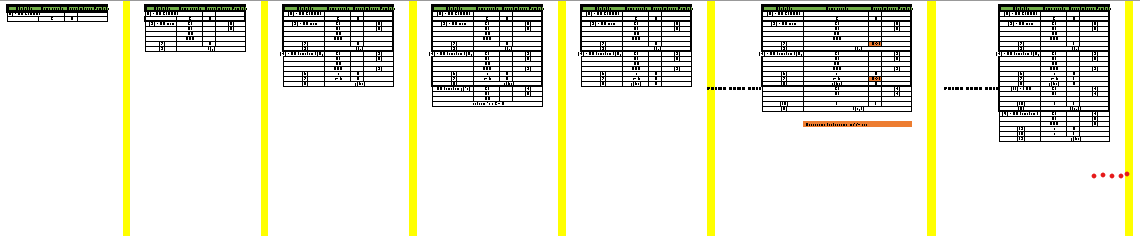
\includegraphics[width=1\textwidth]{Immagini/Partial_RA.png}
	\caption{Parziale soluzione esercizio RA}
	\label{fig:ra}
\end{figure}

\section{EXE 2 - C}
Durante la prova, ho optato per risolvere questo esercizio per ultimo: non è stata una scelta felice, poichè sono arrivato dopo 4 ore di prova a cercare di risolvere un problema all'apparenza complicatissimo ma che, con il senno di poi, si è dimostrato risolvibile (con comunque qualche difficoltà).

\subsection{Non ricorsiva}

\subsection{Ricorsiva senza tail}
\subsection{Ricorsiva CON tail}
\section{EXE 3 - }
\section{EXE 4 - }
\section{EXE 5 - }
\section{EXE 6 - }